% withpage: ページ番号をつける (著者確認用)
% english: 英語原稿用フォーマット
\documentclass{ipsjprosym}
%\documentclass[withpage,english]{ipsjprosym}

\usepackage[dvips]{graphicx}
\usepackage{latexsym}

\begin{document}

% Title, Author %%%%%%%%%%%%%%%%%%%%%%%%%%%%%%%%%
\title{ATS言語を使って不変条件をAPIに強制する}

\affiliate{METASEPI}{METASEPI DESIGN}

\author{岡部 究}{Kiwamu Okabe}{METASEPI}[kiwamu@debian.or.jp]

\begin{abstract}
概要(400字程度) xxx
○○○○○○○○○○○○○○○○○○○○○○○○○○○○○○○
○○○○○○○○○○○○○○○○○○○○○○○○○○○○○○○○○○○○○○○○
○○○○○○○○○○○○○○○○○○○○○○○○○○○○○○○○○○○○○○○○
○○○○○○○○○○○○○○○○○○○○○○○○○○○○○○○○○○○○○○○○
○○○○○○○○○○○○○○○○○○○○○○○○○○○○○○○○○○○○○○○○
○○○○○○○○○○○○○○○○○○○○○○○○○○○○○○○○○○○○○○○○
○○○○○○○○○○○○○○○○○○○○○○○○○○○○○○○○○○○○○○○○
○○○○○○○○○○○○○○○○○○○○○○○○○○○○○○○○○○○○○○○○
○○○○○○○○○○○○○○○○○○○○○○○○○○○○○○○○○○○○○○○○
○○○○○○○○○○○○○○○○○○○○○○○○○○○○○○○○○○○○○○○○
\end{abstract}

\begin{jkeyword}
ATS, 関数型言語, 依存型, 線形型, 組込開発
\end{jkeyword}

\maketitle

% Body %%%%%%%%%%%%%%%%%%%%%%%%%%%%%%%%%
\section{はじめに}

「モノのインターネット (IoT:Internet of Things)」という概念が提唱されています。バスケットボールのような、なんの変哲もないモノがマイクロチップを内蔵してインターネットに接続されるような世界を予想した概念がIoTです。そのIoTによる製造業への経済効果は2850億ドルと試算されています (ガートナー調べ \cite{iot_monoist})。このようなIoTデバイスに対する要件は以下のようなものになるでしょう。

\begin{itemize}
\item インターネットに接続可能なネットワークプロトコルを内蔵
\item 短時間/少工数による設計
\item 個人情報を保管/送信する機能
\item セキュリティへの配慮
\item ネットワーク非対応な機器よりもさらにインテリジェントな機能
\item 安価な価格を実現するため非力なハードウェアの使用
\end{itemize}

一方、現代の組み込み機器はC言語やC++言語を用いて慎重に開発されています。これはこれらの言語を使った開発手法が様々な不具合を誘発するためです。このような不具合の誘発を防ぐために、VDM \cite{vdm} やZ \cite{z_notation} のような形式手法が用いられます。しかし、これらの形式手法はモデルベースのものであり、実際に動作するC言語やC++言語で記述された設計と同期していません。これらのモデルとコードによる設計の同期には、やはり人間の力が必要になります。つまり製品のバージョンを更新する毎にこの形式手法モデルとソースコードを同期させる工数が恒常的に発生してしまいます。

これら慎重な開発はPOSIX API上でのアプリケーション開発と比較にならないほどの工数を必要とします。にもかかわず、IoTデバイスはそのような開発者にPOSIX上のアプリケーションレベルの機能を要求します。このC言語を中心とした開発プロセスは今後持続可能なものなのでしょうか?ソフトウェア理学/工学はこの問題に対して、有効な手を打てないのでしょうか?

本論文ではこの問題に対する1つの解決策としてATS言語 \cite{ats} を紹介します。このATS言語はMLのような関数型言語で、静的な強い型を持ちます。またこの言語は依存型とを持ち、Coq \cite{Coq_manual} のような証明器としても機能します。さらにこの言語の線形型を使うことで、メモリやロックのようなリソースの制御を安全に行なうことができます。ATS言語はC言語を経由して実行バイナリを生成するため、強い型による不変条件の強制は常にソースコードと同期しています。そのため製品のバージョンを数年にわたって更新する場合でも型とソースコードは機械的に同期します。最後にわずか8kBのメモリしか持たないArduino Mega 2560ボード \cite{arduino-mega} 上でATS言語を使って設計したアプリケーションを動作させ、組み込み領域にATS言語を適用可能であることを示します。

\section{既存の組込開発手法の問題}

xxx

\section{ATS言語とは}

xxx

\begin{figure}[h]
\centering
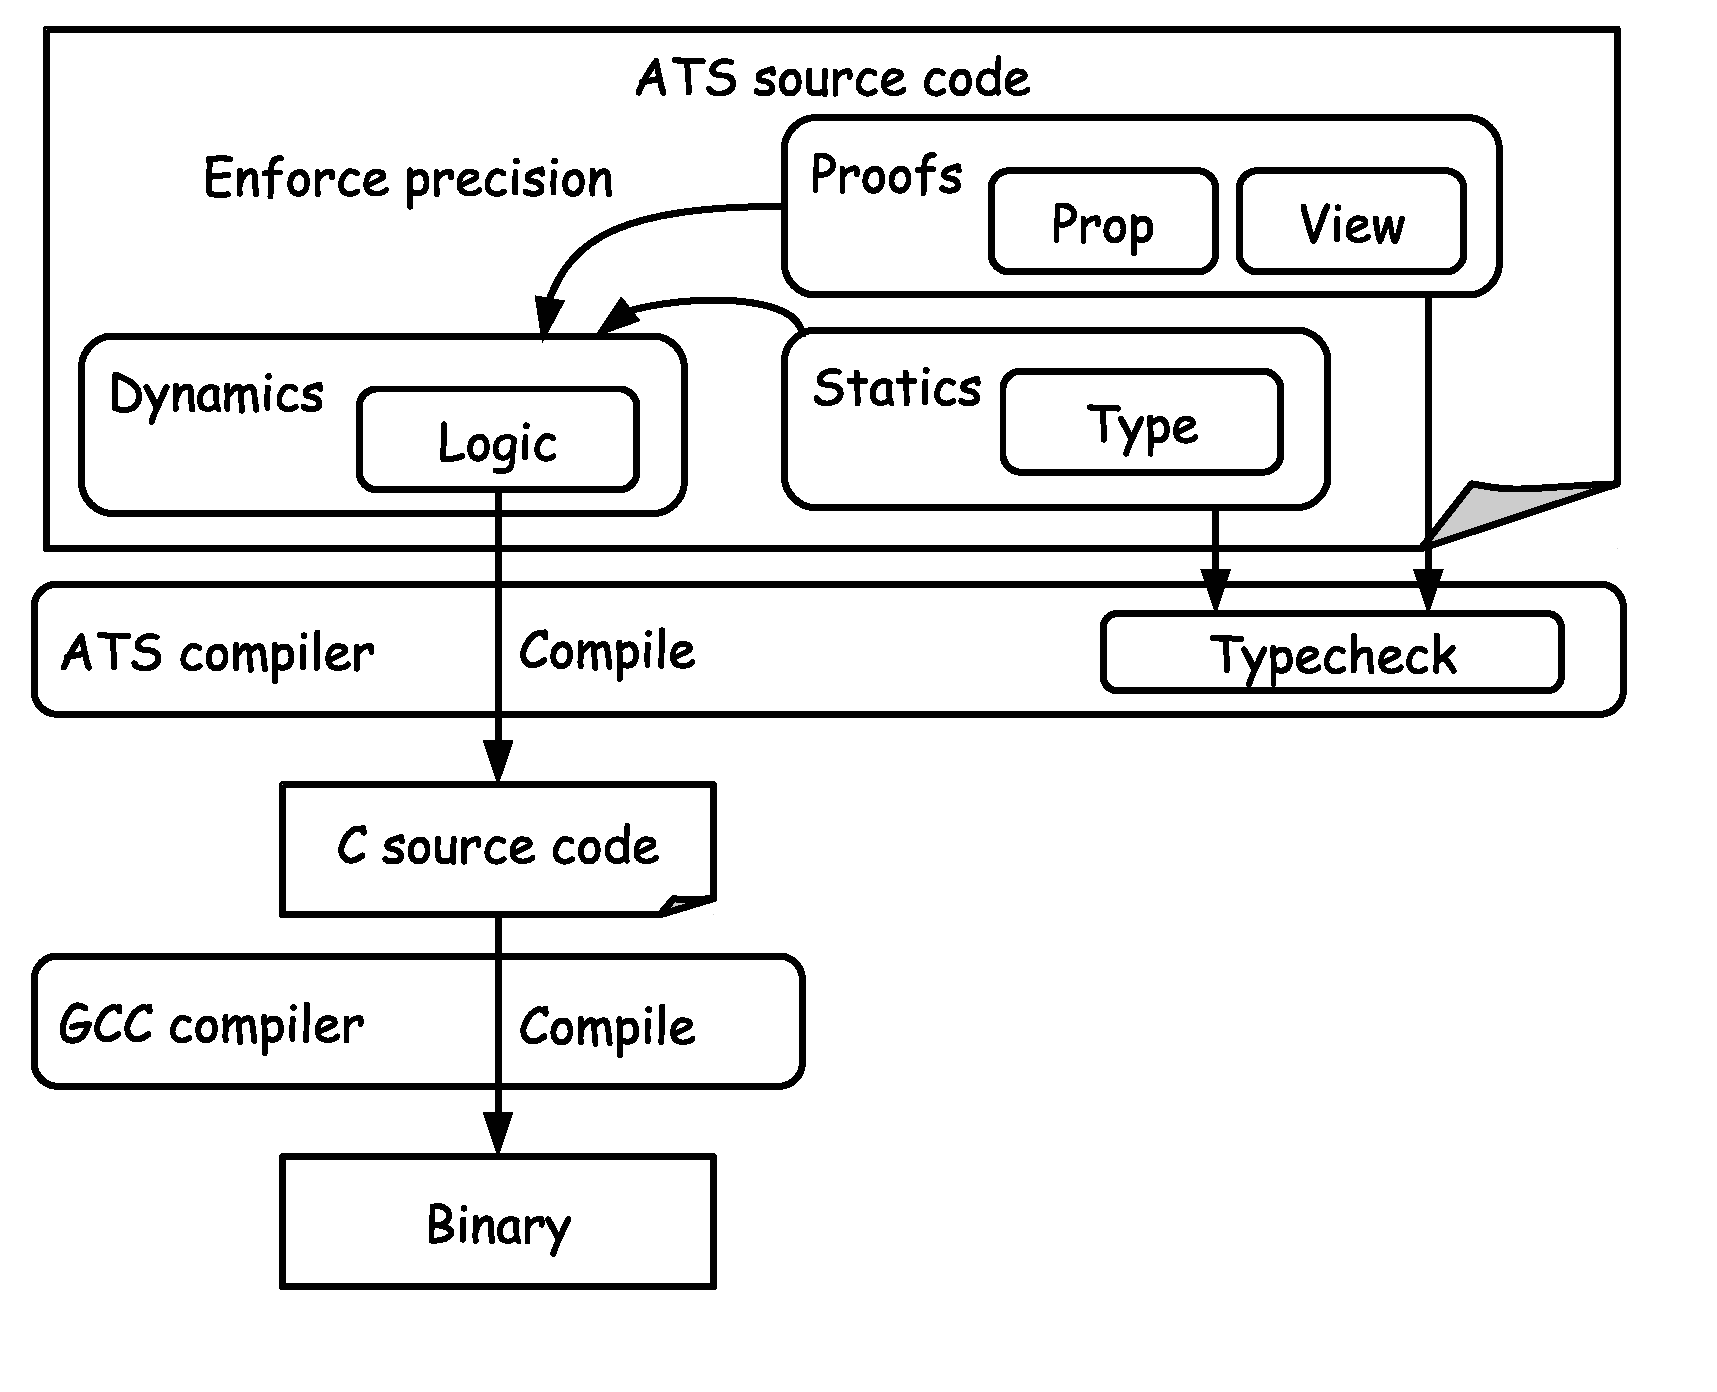
\includegraphics[width=75mm]{draw/flow.eps}
\caption{xxx}
\label{fig:flow}
\end{figure}

\begin{figure}[h]
\centering
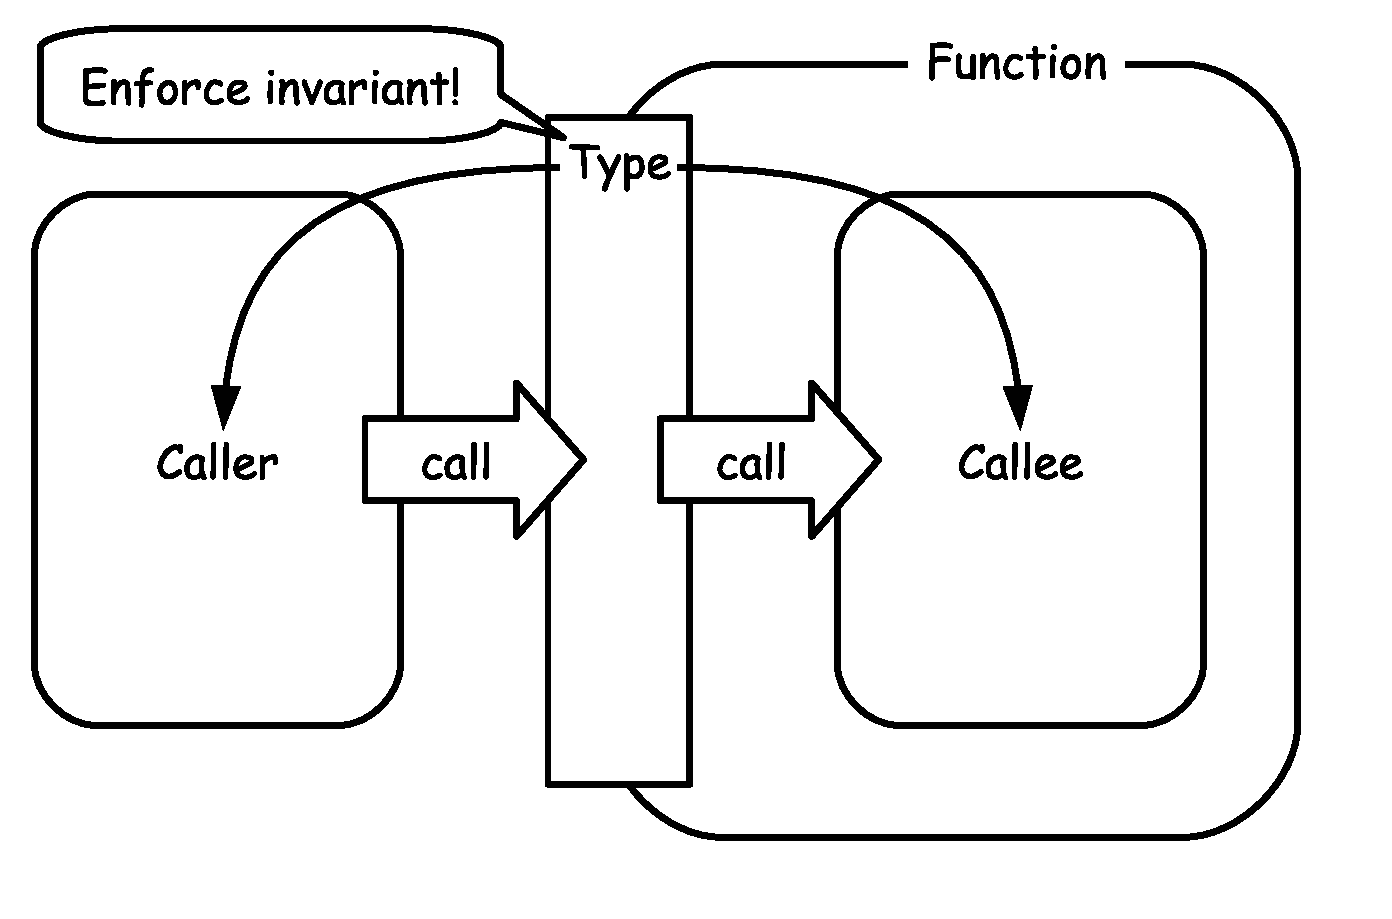
\includegraphics[width=75mm]{draw/enforce_invariant.eps}
\caption{xxx}
\label{fig:enforce_invariant}
\end{figure}

\section{ATSの型について}

xxx

\begin{figure}[h]
\centering
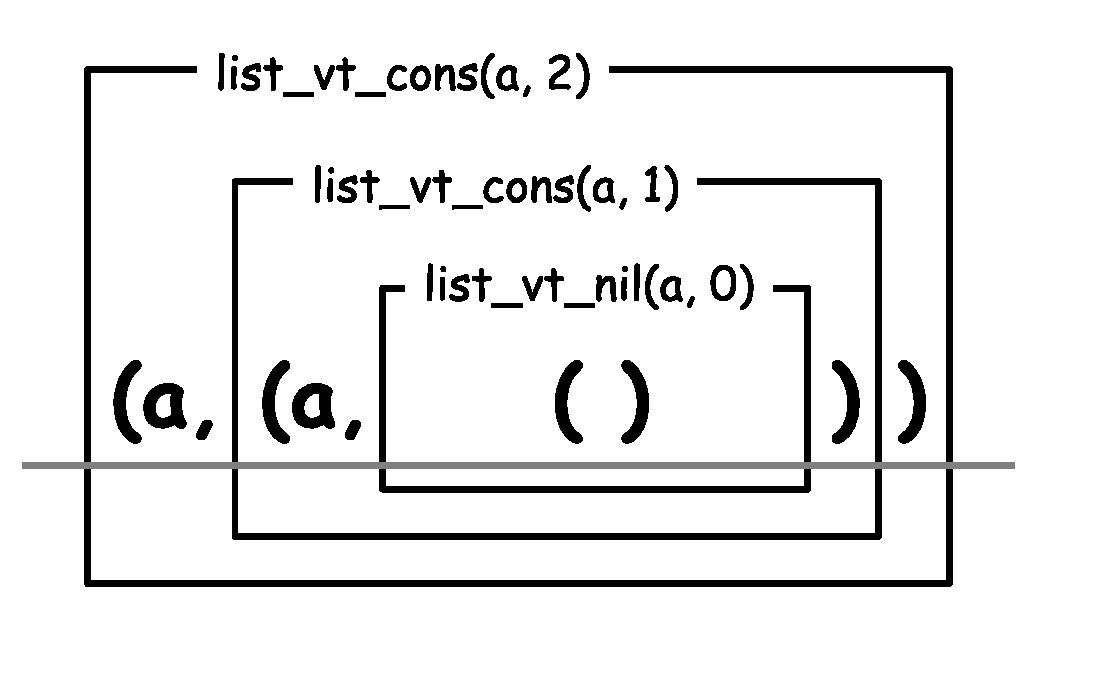
\includegraphics[width=50mm]{draw/list_vt_type.eps}
\caption{xxx}
\label{fig:xxx}
\end{figure}

\begin{figure}[h]
\centering
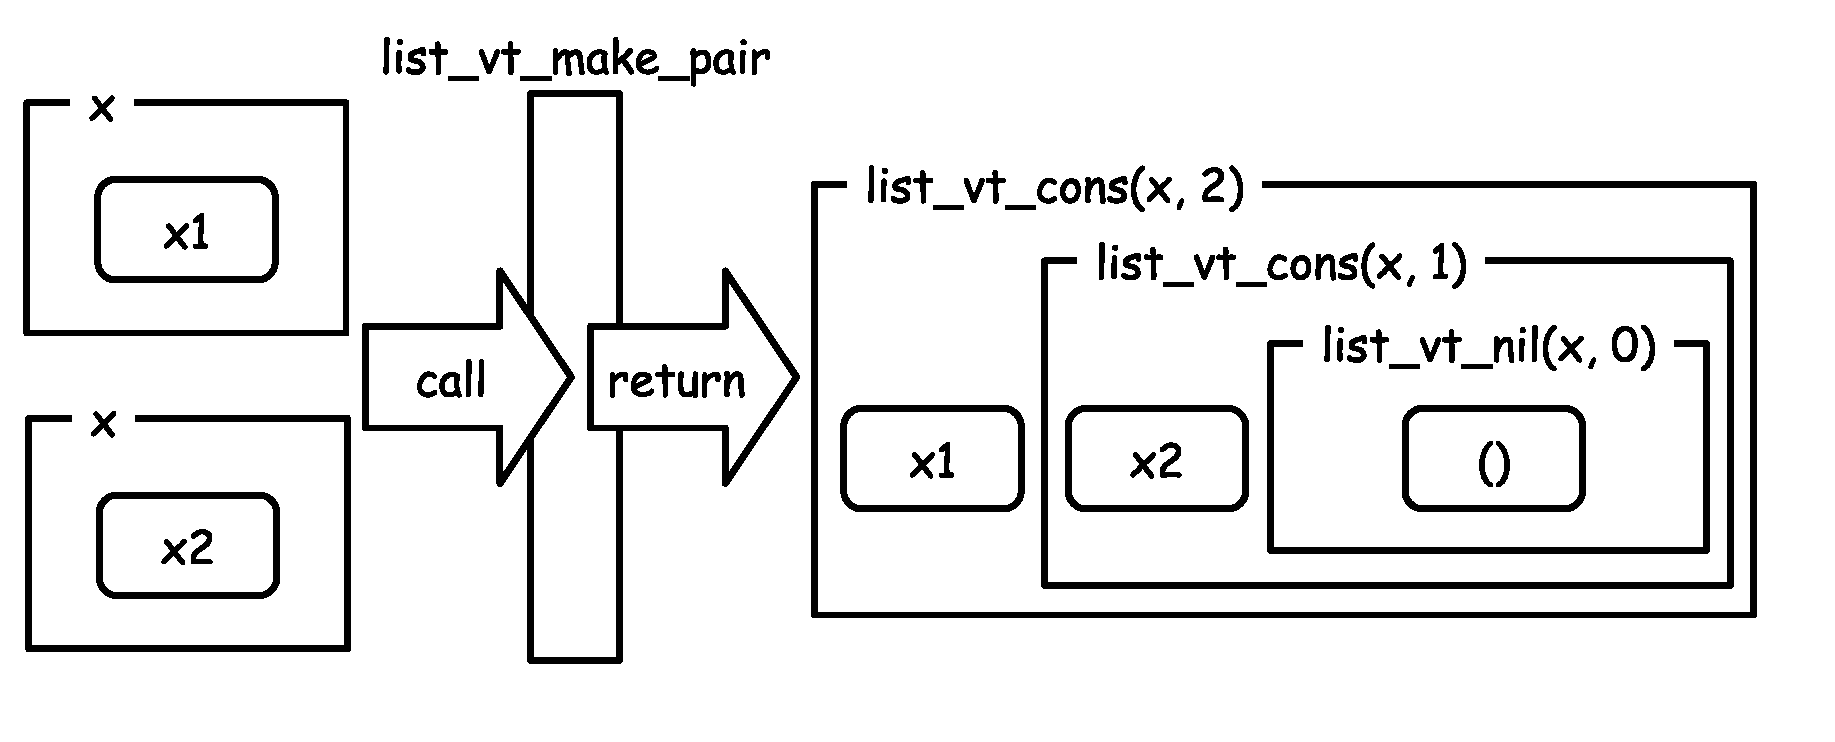
\includegraphics[width=75mm]{draw/list_vt_make_pair.eps}
\caption{xxx}
\label{fig:xxx}
\end{figure}

\begin{figure}[h]
\centering
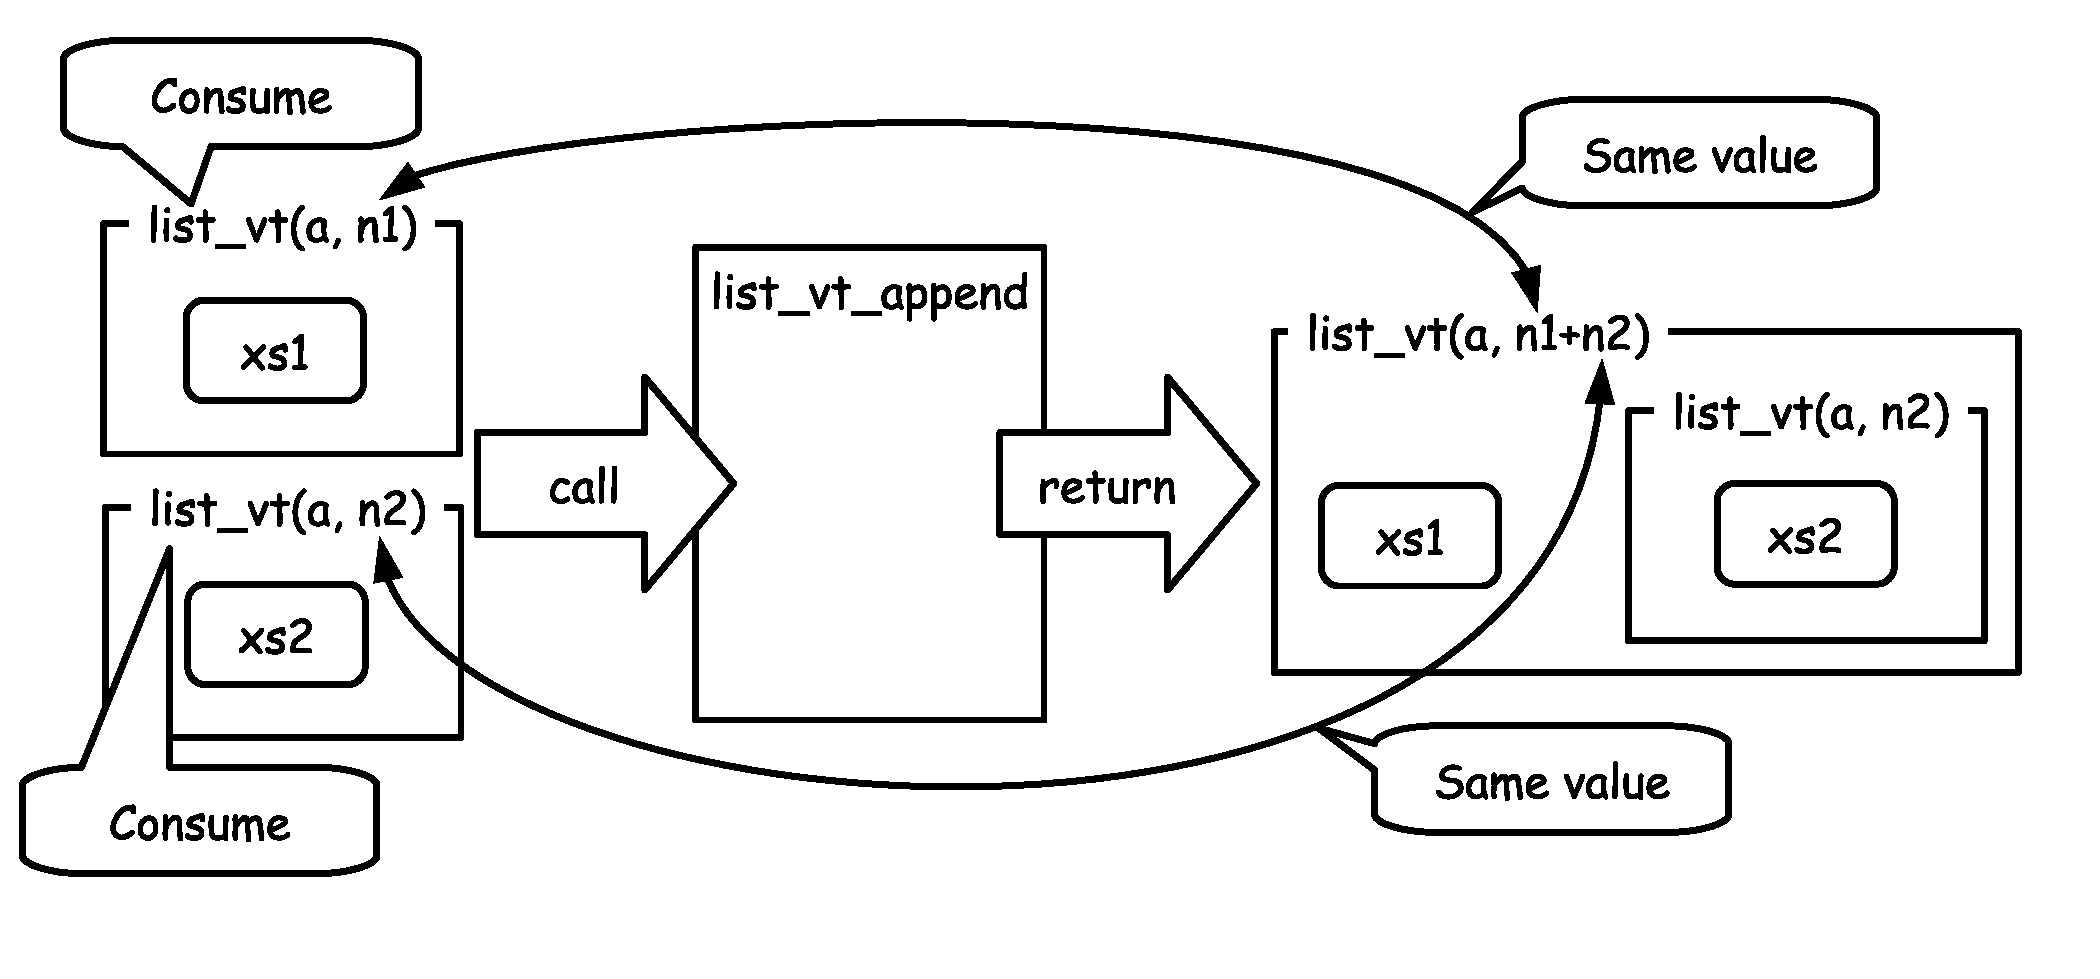
\includegraphics[width=75mm]{draw/list_vt_append.eps}
\caption{xxx}
\label{fig:list_vt_append}
\end{figure}

\begin{figure}[h]
\centering
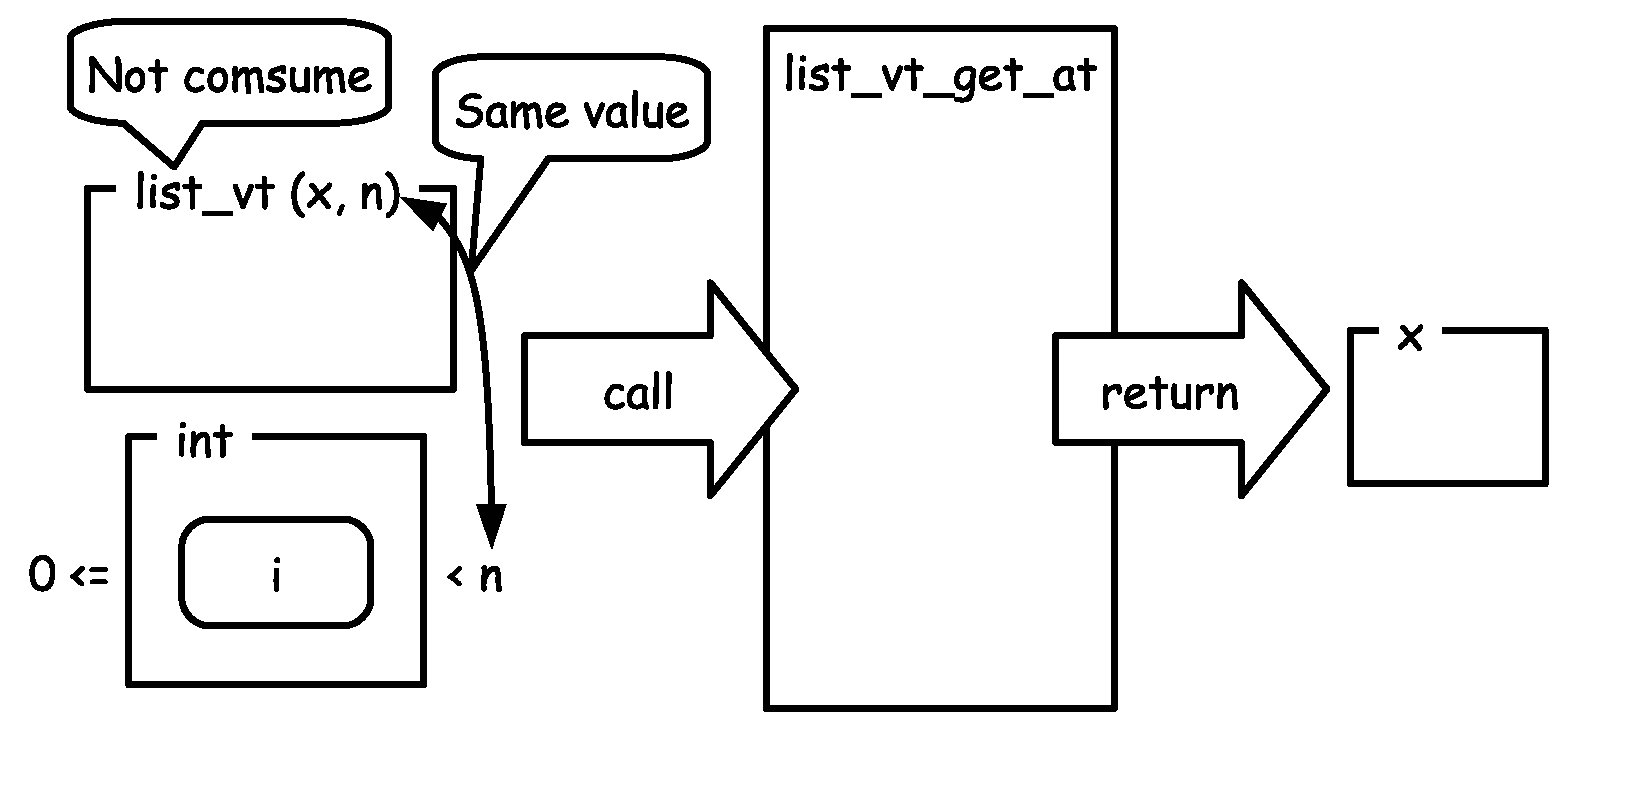
\includegraphics[width=75mm]{draw/list_vt_get_at.eps}
\caption{xxx}
\label{fig:xxx}
\end{figure}

\begin{figure}[h]
\centering
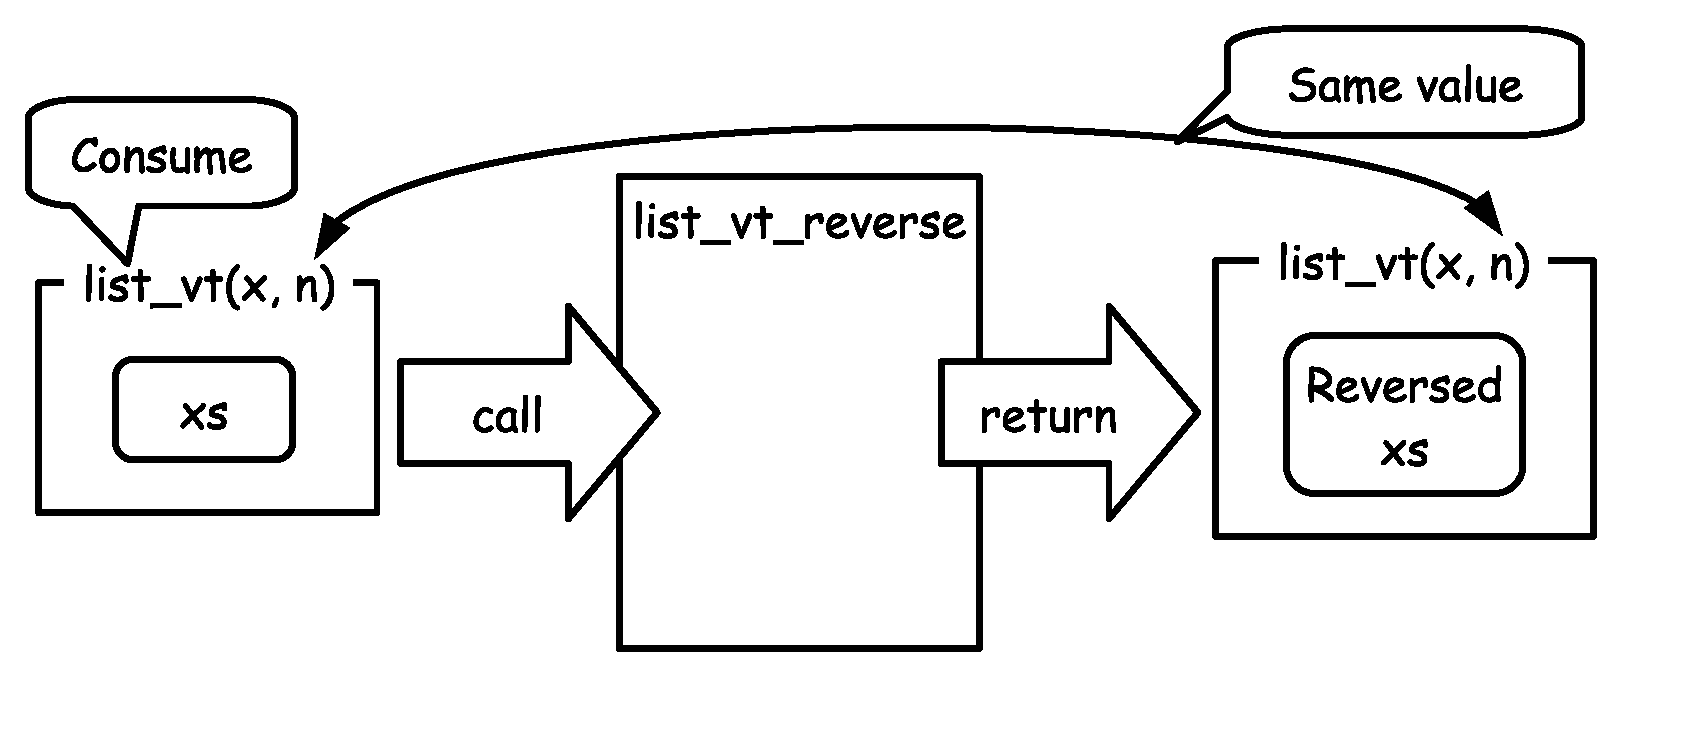
\includegraphics[width=75mm]{draw/list_vt_reverse.eps}
\caption{xxx}
\label{fig:xxx}
\end{figure}

\begin{figure}[h]
\centering
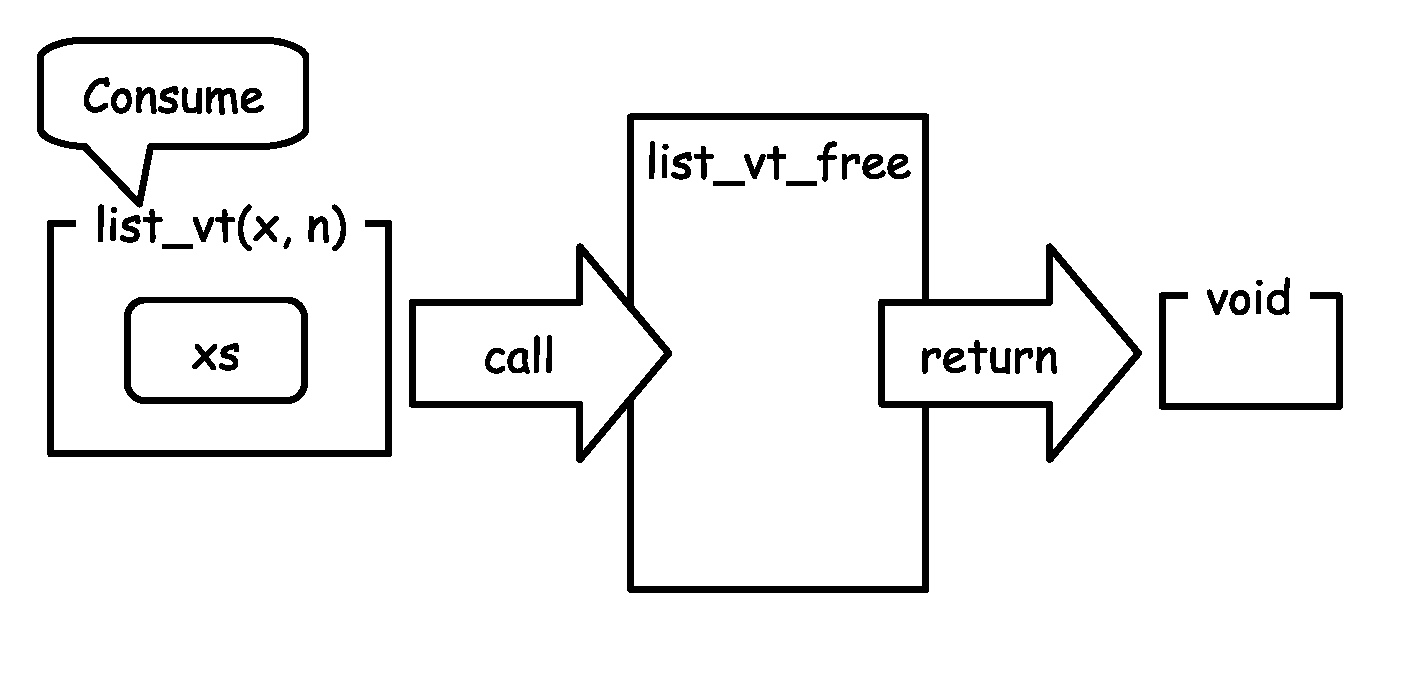
\includegraphics[width=75mm]{draw/list_vt_free.eps}
\caption{xxx}
\label{fig:xxx}
\end{figure}

\section{ArduinoにおけるATSプログラミング}

ATS言語による組み込み開発の適正を評価するために、Arduino Mega 2560ボード上で動作するアプリケーションをATS言語で試作した。このボードは以下のような仕様である。

\begin{description}
  \item[Architecture] 8-bit Harvard architecture
  \item[Microcontroller] ATmega2560
  \item[Flash Memory] 256kB
  \item[SRAM] 8kB
  \item[Clock Speed] 16MHz
\end{description}

本稿を執筆している段階では、さらにメモリの少ないArduino Unoボード \cite{arduino-uno} 上でも同様のアプリケーションの動作に成功している。このアプリケーションのソースコードは \cite{arduino-ats} から入手可能である。

\begin{figure}[h]
\centering
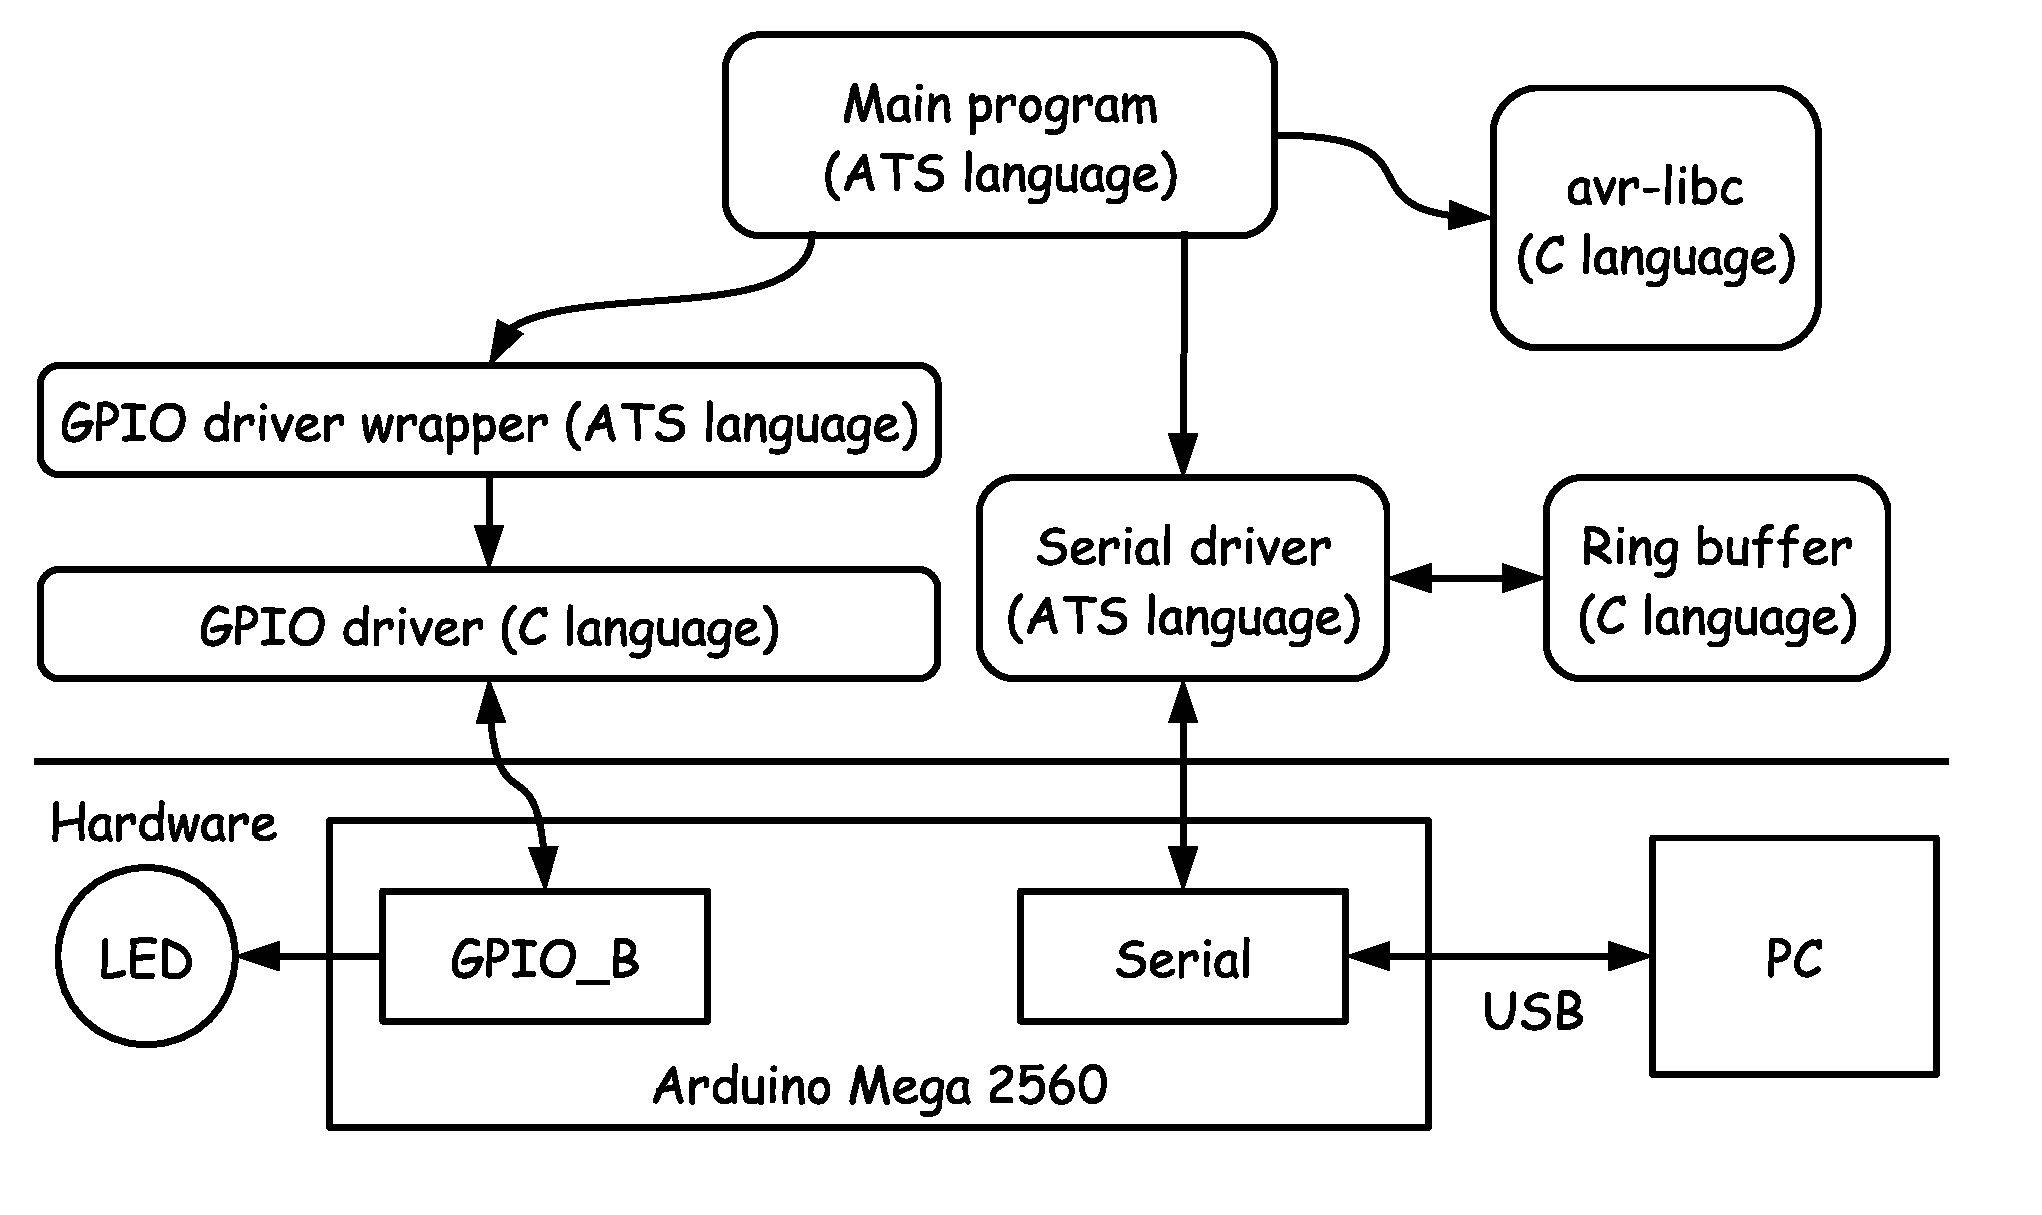
\includegraphics[width=75mm]{draw/demo_ats_arduino.eps}
\caption{Arduino上におけるATSアプリケーション例}
\label{fig:demo_ats_arduino}
\end{figure}

本アプリケーションのアーキティクチャは図\ref{fig:demo_ats_arduino}のようなものである。

xxx

\section{ATSによる組込開発手法の考察}

xxx

\section{結論と今後の課題}

xxx

\begin{acknowledgment}
ATS言語に関して助言をくれたボストン大学の准教授であるHongwei XiとATSコミュニティに感謝する。
\end{acknowledgment}

\begin{QandA}
\item[A] 線形型にvalで別名を作るとどうなるのか?
\item[岡部] 消費される。以下に例を付記する。

\begin{verbatim}
(* コンパイルNG: let valでも線形型が消費されてしまう *)
#include "share/atspre_staload.hats"
implement main0 () = {
  val l1 = list_vt_make_pair<int> (1, 2)
  val l2 = l1
  val () = let val l3 = l2
           in println! l3 end
  val () = free l2
}

(* コンパイルOK: valで線形型が消費される *)
#include "share/atspre_staload.hats"
implement main0 () = {
  val l1 = list_vt_make_pair<int> (1, 2)
  val l2 = l1
  val () = println! l2
  val () = free l2
}
\end{verbatim}

\item[B] リングバッファをATSで書くのは難しいのか?
\item[岡部] 公式ドキュメントに例があるぐらいなので、リングバッファ自体は簡単。しかし、スレッドセーフ化や再入可能にするのはそれなりに難しい。
\item[C] マルチスレッドを生かしたプログラミングをするにはどうすれば良いか?
\item[岡部] セッションのようなものを作る。例えばmutexのロックと開放では、その間にセッションが存在すると考えることができる。セッションの間は静的な型を効果的に使うことができる。
\item[D] ATSに辿りつくまでのMetasepiプロジェクトの歴史について
\item[岡部] ATSを使ったイテレーションは2番目。1番目ではHaskell言語とjhcコンパイラを使っていた。Haskellの欠点は、メモリ領域の扱いがルーズ、マシン表現と言語表現にギャップがあること。ATSの欠点は、抽象化の機能が弱いこと。
\end{QandA}

% BibTeX を使用する場合 %%%%%%%%%%%%%%%%%%%%%%%%%%%%%%%%%
\bibliographystyle{ipsjsort}
\bibliography{../bibtex/reference,../bibtex/jreference}

\end{document}
